\begin{itemize}[noitemsep,topsep=2pt,parsep=2pt,partopsep=2pt,leftmargin=*]
\item \textbf{Why do we need to perform model simplification in the era of (almost) infinite computation power?}:


Model Simplification is essential even when computation power has increased dramatically \cite{Stolt2005}, because:
	\begin{itemize}[noitemsep,topsep=2pt,parsep=2pt,partopsep=2pt,leftmargin=*]
	\item more complex problems can be solved
	\item more design iterations can be performed
	\end{itemize}
	
	
\item \textbf{Which Domain needs Midsurface the most?}: 

Thin-walled components are widely used in aerospace, automotive and many other industries (Figure \ref{fig:litsurvey:ThinWallApplications}) due to their advantages of material/cost/energy saving and easy manufacturability.  Injection Moulding parts are most complex due to draft and have most demand for better Midsurface. Here even surface does not get generated, then connections. Sheet Metal parts are relatively easy, create surfaces but fail in connections. So it is better to start with Sheet Metal parts and then attempt generic or injection molding parts

%%\bigskip


	\begin{figure} [!h]
		\centering
		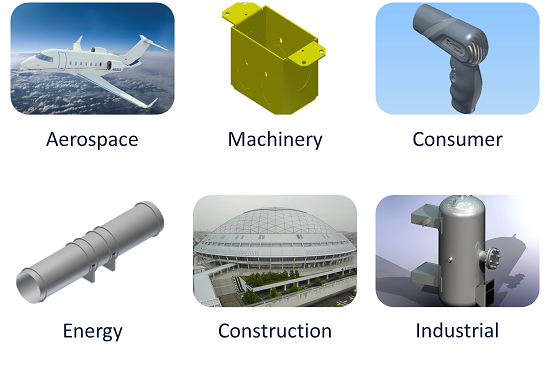
\includegraphics[width=0.6\linewidth]{..//Common/images/ThinWallApplications}
		\caption{Thin Wall Applications (Source: Autodesk \cite{SheetMetalAutodesk})}
		\label{fig:litsurvey:ThinWallApplications}
	\end{figure}
	
%%\bigskip


\item \textbf{Which input format is most suitable?}: 

Feature based CAD (Brep) models are far richer has they application specific sub-volumes apart from geometry and topology. This research does not deal with Mesh, Voxel, plain Brep, CSG model. Features can be live via API or through some neutral export format  \cite{Dabke1994}.

\item \textbf{What are advantages of Midsurface wrt Shell Elements?}:
	\begin{itemize}[noitemsep,topsep=2pt,parsep=2pt,partopsep=2pt,leftmargin=*]
	\item Shell Elements are more efficient than 3D elements for Thin Wall (Figure \ref{fig:litsurvey:shellsolidelems})
	\item Experimentation with just thickness can be done, for 3D elements remeshing would be needed
	\item For 3D elements minimum 3 layers would be needed which is not feasible for really thin portions
	\item Solid elements may show locking under bending dominated loading
	\end{itemize}
		
		%%\bigskip

	\begin{figure} [!h]
		\centering
		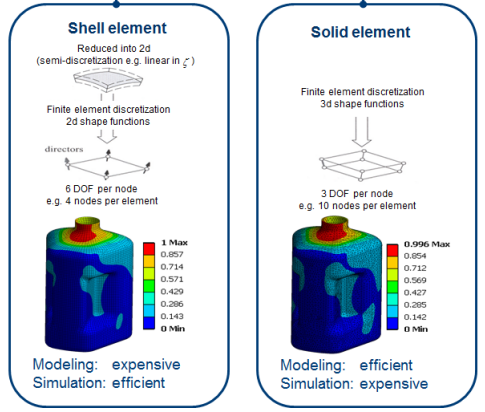
\includegraphics[width=0.6\linewidth]{..//Common/images/ShellSolidElems}
		\caption{Comparative Analysis of Shell Solid Elements (Source: Cosmos \cite{Cosmos2006})}
		\label{fig:litsurvey:shellsolidelems}
	\end{figure}
	
%%\bigskip


	
\item \textbf{Why compute surface at the Mid and not just use one side?}: 

For thin-walled parts, instead of computing Midsurface, the obvious choice is to use either of the top/bottom surfaces to place the shell elements. But these surfaces are not good choices and we have to go for the Midsurface as it truly represents the part. In case of assemblies or connections midsurfaces connect better across the parts. Also thickness-data/material is represented well as it distributed on both sides in case of Midsurface. For thin-walled parts, the choice of surface can be either outer, inner or somewhere in the middle. In the first two cases, surfaces are ready and no new computation is needed. But still midsurface seems to be a preferred option. 

\begin{itemize}[noitemsep,topsep=2pt,parsep=2pt,partopsep=2pt,leftmargin=*]
\item \textbf{Geometric Consideration}:
	
Defining a mesh of thin shell elements on a part's Midsurface may yield better results than defining a mesh on either the part's outer or inner surfaces. This is because the mesh on the Midsurface  gives a closer approximation of the volume of the part \cite{SDRC2009}.
	
%%\bigskip


	\begin{figure} [!h]
		\centering
		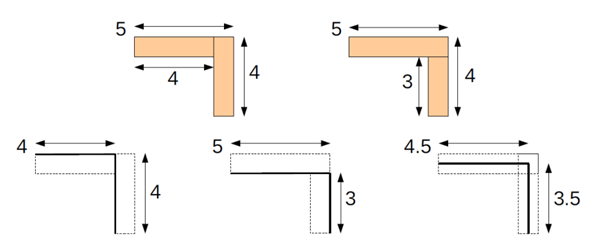
\includegraphics[width=0.8\linewidth]{..//Common/images/OneSide}
		\caption{Need for Midsurface Compared to One Side (Source: Smit \cite{Smit2011})}
		\label{fig:litsurvey:oneside}
	\end{figure}
	
%%\bigskip


\item \textbf{Analysis Consideration}:
If you choose a surface for the shell mesh placement that isn't at the Midsurface of the part, the analytical part will differ from the CAD part by $1/2$  a wall thickness everywhere.  In some areas, your part may analyze as larger than you expected, in others, smaller.  It is comforting to note that the higher the part's aspect ratio or the better candidate a part is for a shell mesh, the less shell surface placement matters. In the grand scheme of things, on a system as large as that garbage truck body shown earlier, $1/2$   wall thicknesses either way will not impact the results in a measurable way. However, as a part approaches the gray zone where it could be modeled as shells or solids, Midsurface placement of the shell becomes important \cite{Cosmos2006}.
\end{itemize}

\item \textbf{What are the issues with prominent medial generation methods?}: 
	\begin{itemize}[noitemsep,topsep=2pt,parsep=2pt,partopsep=2pt,leftmargin=*]
	\item MAT: unsuitable as it creates branches, needs pruning. This can be used in 2D profile case along with Parametric and/or tringularization (chordal method) for connections.
	\item MA: Face pairing is complex
	\item Feature based: So far Sweep based (Extrude, Revolve, Sweep) and primitives like parallelepiped, cylinder, wedge, Pad, Pocket as individual features have been tried. But a generic method, taking care of interactions is missing.
	\item Errors: Gaps, missing surfaces, overlapping surfaces etc. (Fig. \ref{fig:litsurvey:gaps})
	
%%\bigskip


		\begin{figure} [h]
		\centering
		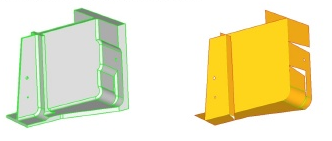
\includegraphics[width=0.6\linewidth]{..//Common/images/MidsurfaceGaps}
		\caption{Midsurface Gaps (Source: Austreng \cite{Austreng2007})}
		\label{fig:litsurvey:gaps}
	\end{figure}
	
%%\bigskip


	\item Commercial:
		\begin{itemize}[noitemsep,topsep=2pt,parsep=2pt,partopsep=2pt,leftmargin=*]
		\item For Sheet Metal, majority of surfaces come out fine. Only problems are at the connections, which we do on Mesh. Tubular structures (such as Motorcycle chassis) have quite a few connection problems. 
		\item For plastic parts, problems are many. Variable thickness, steps, small but elongated features, are main causes of not getting good Midsurface.  Automatic Midsurface is almost not useful.
	\end{itemize}

	\end{itemize}
	
\end{itemize}	

Relevant findings/quotes by various researchers are:
	\begin{itemize}[noitemsep,topsep=2pt,parsep=2pt,partopsep=2pt]
	\item {\em``There is a definite need for a dimensional reduction capability that is more powerful and easier to use than those currently available in the market. Such a capability should deliver an automated scheme for handling cases that have traditionally caused problems for algorithms in this field.'' - Stanley Felix, 2010 } \cite{Stanley2010}
	\item {\em ``Much of research is yet to be done, use of symmetry, various features, various abstractions are not yet handled.'' - Matt Smit, 2011 } \cite{Smit2011}
	\item {\em  ``Valid mid-surfaces may not be abstracted, and mid-surfaces which are abstracted may not be useful in practice as solid models become increasingly complex.''- Yoonhwan Woo, 2013 \cite{Woo2013}}
	\item {\em  ``Mid-surface repair is tedious and manual'' - MSc at the launch of  semi-automatic `Smart Midsurface', 2015 \cite{Msc2015}}
	\end{itemize}
	

